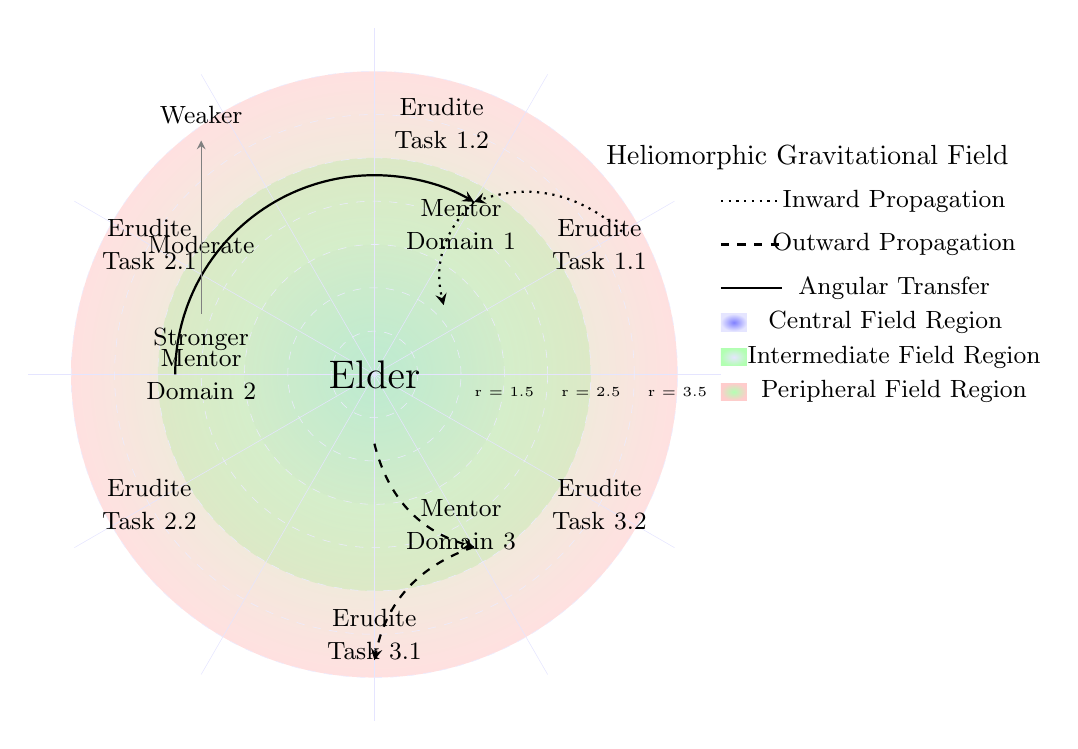
\begin{tikzpicture}[scale=1.1]
  % Define colors
  \colorlet{eldercore}{blue!50}
  \colorlet{elderfield}{blue!10}
  \colorlet{mentorfield}{green!30}
  \colorlet{eruditefield}{red!20}
  \colorlet{elderborder}{blue!50}
  \colorlet{mentorborder}{green!50}
  \colorlet{eruditeborder}{red!50}
  
  % Draw gravitational field using more continuous gradient shading
  \shade[inner color=eldercore, outer color=elderfield, opacity=0.8] (0,0) circle (1.5);
  \shade[inner color=elderfield, outer color=mentorfield, opacity=0.7] (0,0) circle (2.5);
  \shade[inner color=mentorfield, outer color=eruditefield, opacity=0.6] (0,0) circle (3.5);
  
  % Add subtle field lines for gravitational effect - make them more radial
  \foreach \angle in {0,30,...,330}
    \draw[elderborder!20, very thin] (0,0) -- (\angle:4);
    
  \foreach \r in {0.5,1.0,...,3.5}
    \draw[elderborder!15, dashed, very thin] (0,0) circle (\r);
  
  % Add Elder, Mentor, Erudite labels
  \node at (0,0) {\Large Elder};
  
  % Mentor text nodes at different angles
  \node[text width=1.5cm, align=center] at (60:2) {\small Mentor\\Domain 1};
  \node[text width=1.5cm, align=center] at (180:2) {\small Mentor\\Domain 2};
  \node[text width=1.5cm, align=center] at (300:2) {\small Mentor\\Domain 3};
  
  % Erudite text nodes at different angles
  \node[text width=1.5cm, align=center] at (30:3) {\small Erudite\\Task 1.1};
  \node[text width=1.5cm, align=center] at (75:3) {\small Erudite\\Task 1.2};
  \node[text width=1.5cm, align=center] at (150:3) {\small Erudite\\Task 2.1};
  \node[text width=1.5cm, align=center] at (210:3) {\small Erudite\\Task 2.2};
  \node[text width=1.5cm, align=center] at (270:3) {\small Erudite\\Task 3.1};
  \node[text width=1.5cm, align=center] at (330:3) {\small Erudite\\Task 3.2};
  
  % Arrows for Knowledge Flow - Modified to show continuous influence patterns
  % Inward propagation (abstraction)
  \draw[->, thick, dotted, >=stealth, draw=black] (30:3.3) to[bend right] (60:2.3);
  \draw[->, thick, dotted, >=stealth, draw=black] (60:2.3) to[bend right] (0.8,0.8);
  
  % Outward propagation (specialization) - with inverse-square indicator
  \draw[->, thick, dashed, >=stealth, draw=black] (0,-0.8) to[bend right] (300:2.3);
  \draw[->, thick, dashed, >=stealth, draw=black] (300:2.3) to[bend right] (270:3.3);
  
  % Angular dynamics (cross-domain transfer)
  \draw[->, thick, >=stealth, draw=black] (180:2.3) arc (180:60:2.3);
  
  % Legend
  \node[align=left] at (5,2.5) {Heliomorphic Gravitational Field};
  \draw[thick, dotted, >=stealth, draw=black] (4,2) -- (4.7,2);
  \node[align=left, font=\small] at (6,2) {Inward Propagation};
  \draw[thick, dashed, >=stealth, draw=black] (4,1.5) -- (4.7,1.5);
  \node[align=left, font=\small] at (6,1.5) {Outward Propagation};
  \draw[thick, >=stealth, draw=black] (4,1) -- (4.7,1);
  \node[align=left, font=\small] at (6,1) {Angular Transfer};
  
  % Field gradient indicators
  \shade[inner color=eldercore, outer color=elderfield] (4,0.5) rectangle (4.3,0.7);
  \node[align=left, font=\small] at (5.9,0.6) {Central Field Region};
  \shade[inner color=elderfield, outer color=mentorfield] (4,0.1) rectangle (4.3,0.3);
  \node[align=left, font=\small] at (6.0,0.2) {Intermediate Field Region};
  \shade[inner color=mentorfield, outer color=eruditefield] (4,-0.3) rectangle (4.3,-0.1);
  \node[align=left, font=\small] at (6.0,-0.2) {Peripheral Field Region};
  
  % Field strength indicators
  \node[font=\small] at (-2.0,0.4) {Stronger};
  \node[font=\small] at (-2.0,1.5) {Moderate};
  \node[font=\small] at (-2.0,3.0) {Weaker};
  \draw[->, >=stealth, draw=black!50] (-2.0,0.7) -- (-2.0,2.7);
  
  % Field radius markers
  \node[font=\tiny] at (1.5,-0.2) {r = 1.5};
  \node[font=\tiny] at (2.5,-0.2) {r = 2.5};
  \node[font=\tiny] at (3.5,-0.2) {r = 3.5};
\end{tikzpicture}